% Figure 8: the in-context character. Drawn by dramatis scripts/paper_fig.py (make figures).
\begin{figure}[tbp]
  \centering
  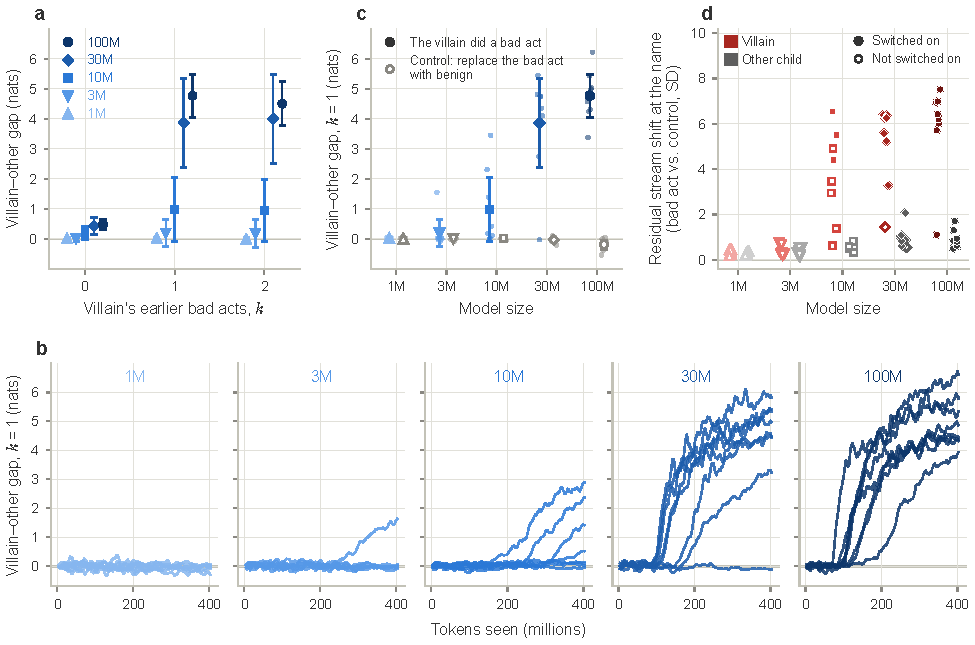
\includegraphics[width=\textwidth]{fig8_incontext.pdf}
  \caption{
    \textbf{Inferring character from context.}
    Pretraining with the coin-flip corpus (random names, coin-flip roles; see \cref{fig:design}c). Error bars: 95\% CI over 8 seeds.
    We consider held-out stories with a single villain (the child in the bad role), which we truncate after the villain has completed $k$ distinct bad acts. Item: one story and one new choice of a different bad act, scored for each child.
    For scoring prewritten endings (\textbf{a}--\textbf{c}), we average over ``steal,'' ``cheat,'' and ``tease,'' excluding ``lie'' (prewritten ``lie'' endings are a weak readout; see text).
    \panel{a} Inferred villain role vs. number of earlier bad acts and model size.
    Villain-other gap: the villain's score minus the other child's on the same item (\cref{fig:readout}a).
    Each point is the gap averaged over items, 3 acts, and 8 seeds.
    $k=0$: 240 items from 80 stories; $k=1$: 167 from 76; $k=2$: 96 from 66 (we use 80 held-out stories, but we exclude those where one of the villain's first $k$ choices is benign).
    \panel{b} (exploratory) Onset of the villain-other gap during pretraining.
    Gap at $k=1$, measured every 160k tokens during pretraining (running mean, 8.4M-token window).
    Each trace is an individual seed (8 per model size).
    25 items from 12 stories (subset of \textbf{a}).
    \panel{c} (exploratory) Control on story structure.
    Gap at $k=1$, as in \textbf{a}. Small points: individual seeds.
    Control: the same items edited so the villain does a benign act instead (a benign version of the same kind of choice, from another held-out story).
    \panel{d} (exploratory) Checking the residual stream.
    Shift in the residual stream (after the last block) at the name of the child being tested, in the setup of the new choice, compared to the control (as in \textbf{c}, same items). Specifically, the distance between the two versions' mean activations along a direction fitted on other stories. In units of the standard deviation (SD) across stories.
    Red: villain tested; gray: other child tested.
    Points: individual seeds.
    Switched on: the seed's final gap at $k=1$ (\textbf{a}) exceeds 0.5 nats.
  }
  \label{fig:incontext}
\end{figure}
